%=====================================================
%====== If you are new to LaTeX, this website ========
%======     will be your new best friend:     ========
%======   http://en.wikibooks.org/wiki/LaTeX  ========
%======   Template created by Jonathan Blair  ========
%=====================================================



%=====================================================
%============ Controls ===============================
%=====================================================

%\documentclass[12pt,letterpaper,onecolumn]{article}
\documentclass[11pt,letterpaper,onecolumn]{article}
%\documentclass[10pt,letterpaper,onecolumn]{article}  % not recommended
%\documentclass[12pt,letterpaper,twocolumn]{article}
%\documentclass[11pt,letterpaper,twocolumn]{article}
%\documentclass[10pt,letterpaper,twocolumn]{article}


\usepackage{amsmath}
\usepackage{graphicx}
\usepackage{url}
\usepackage{textgreek}
\usepackage{float}
\usepackage{booktabs}
%\graphicspath{{path-to-folder-containing-necessary-graphics}{other folder as necessary}}


%=====================================================
%============ \begin{document} =======================
%=====================================================

\begin{document}

%=====================================================
%============ Title ==================================
%=====================================================

\title{\bf Observation of the Properties and Behavior of Diodes}
%\title{\Large\bf Larger, Bolded Title}

%=====================================================
%============ Author =================================
%=====================================================
\author{
 Jairo Portillo \\*
  \\*
 PHY 338K Electronic Techniques \\*
 Department of Physics \\*
 The University of Texas at Austin \\*
 Austin, TX 78712, USA
}
\date{February 18, 2016}

%\address{The University of Texas, Austin, Texas, 78712}

\maketitle

%=====================================================
%============ Abstract ===============================
%=====================================================

\begin{abstract}

In this lab, we will explore the properties of diodes and how they influence signals and interact with other circuit elements. First, we will explore the diode's characteristics of rectifying a signal. Then we use this property to form a DC signal and limit the wave signal. Finally, we will use a light emitting diode diode and determine its forward and reverse bias position.   

\end{abstract}

%=====================================================
%============ Body of the article ==========================
%=====================================================

%=====================================================
%============ Section ==================================
%=====================================================

\section{Preperation}

In order to prepare for this lab, we must review the behavior of diodes. Diodes are a non linear circuit element. Diode allow current to pass easily while in forward bias which is when current flow from the anode to the cathode. When the diode is in reverse, that is when the current flows from the cathode to the anode, current can not flow until it reaches the reverse break down voltage. Diodes are used in rectifier which changes AC to DC. The behavior of diodes in rectifiers in the main focus for this lab. 

\section{Lab work}

\subsection{Apparatus}

\begin{figure}[H]
    \hspace*{-2cm}
    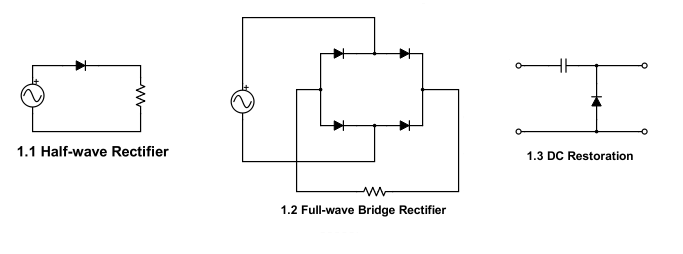
\includegraphics[scale = .9]{Circuits.png}
    \caption{Some of the circuits that will be used in this lab.}
    \label{fig:Cir}
\end{figure}

This lab will use a signal generator and an oscilloscope. The oscilloscope will not me grounded and the signal generator will be the ground for the circuits that require it. Due to the design of the oscilloscope with the three port connected with a plate, an external trigger will not be used. This is due the fact the external trigger is grounded and will disrupt the output signal. We will also use four diodes, a $2.66\Omega$ and $5\Omega$ resistors,a $.483\mu C$ capacitor, and a 10V zener diode. We will recreate the circuit configurations as seen in Figure \ref{fig:Cir}. For Figure \ref{fig:Cir}.1 and Figure \ref{fig:Cir}.2, the voltage across the load resistor is what will be measured. 

\subsection{Data Collection}

\subsubsection{Diode Characteristics}

The first portion of this lab is to observe characteristics of a diode in various rectifier circuit configurations. We first explore the the capabilities of the half wave rectifier as seen in Figure \ref{fig:Cir}.1. In a half wave rectifier we expect the negative portion of the sine wave to flat line. To observe this we pass a 1KHz 20V peak to peak signal through circuit in Fig. 1.1 and see the output voltage drop to 9.8V peak to peak as expected. The negative of the portion of the signal is also flat lined as expected. Reducing the input to 1V peak to peak maintains the expected behavior.

\begin{figure}[H]
    \hspace*{-2.5cm}
    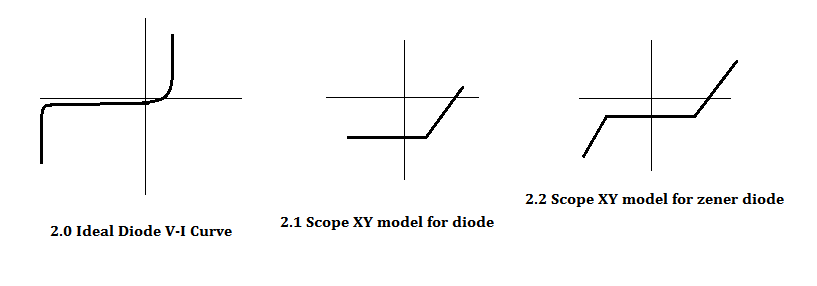
\includegraphics[scale = .8]{graphs.png}
    \caption{2.1) Graph of the ideal diode behavior.
    2.2) and 2.3) models of what was observed on the oscilloscope.}
    \label{fig:graph}
\end{figure}

We then observed the voltage and current relation using the oscilloscope's x-y mode. For a solid state diode, we observed a graph such as that on fig. 2.1. This demonstrated that the diode was in forward bias. We then placed the zener diode in it's place and then observed fig. 2.2. The zener diode demonstrated the forward and reverse bias behavior as expected from an ideal diode in fig 2.0. 

A full wave rectifier as in fig 1.2, was used in order to verify the expected behavior of the configuration. The full wave rectifier gives an out put signal similar to that of the absolute value of the wave but without the sharp peaks at the nodes. The nodes are instead flat lines. The observed output followed the model of what was expected. Replacing the load resistor of fig 1.2 with a low pass circuit, we observed a ripple voltage. When the capacitance was increased, increasing the time constant, the ripple effect decreases. In other words the ripple effect become more like a DC flat line signal and the time constant increases. 

\subsubsection{Diode Wave Shaping and Clamp Circuits}

The full capabilities of a diodes ability to turn AC to DC was examined in this portion of the lab. We formed a DC restoration circuit as in fig. 1.3 with a 5K$\Omega$ resistor. The AC signal we passed through the circuit was "restored" to a DC signal due to the configuration. The diode limiter circuit however also converted the AC to DC but it was influences by the offset of the AC signal. When the 1V AC signal was offset below the ground, the DC signal was at -400mV. When the signal intercepts, the DC signal was at 600mV and when above the DC signal peaked at 800mV.   

\subsubsection{Light Emitting Diode (LED)}

\begin{figure}[H]
    \centering
    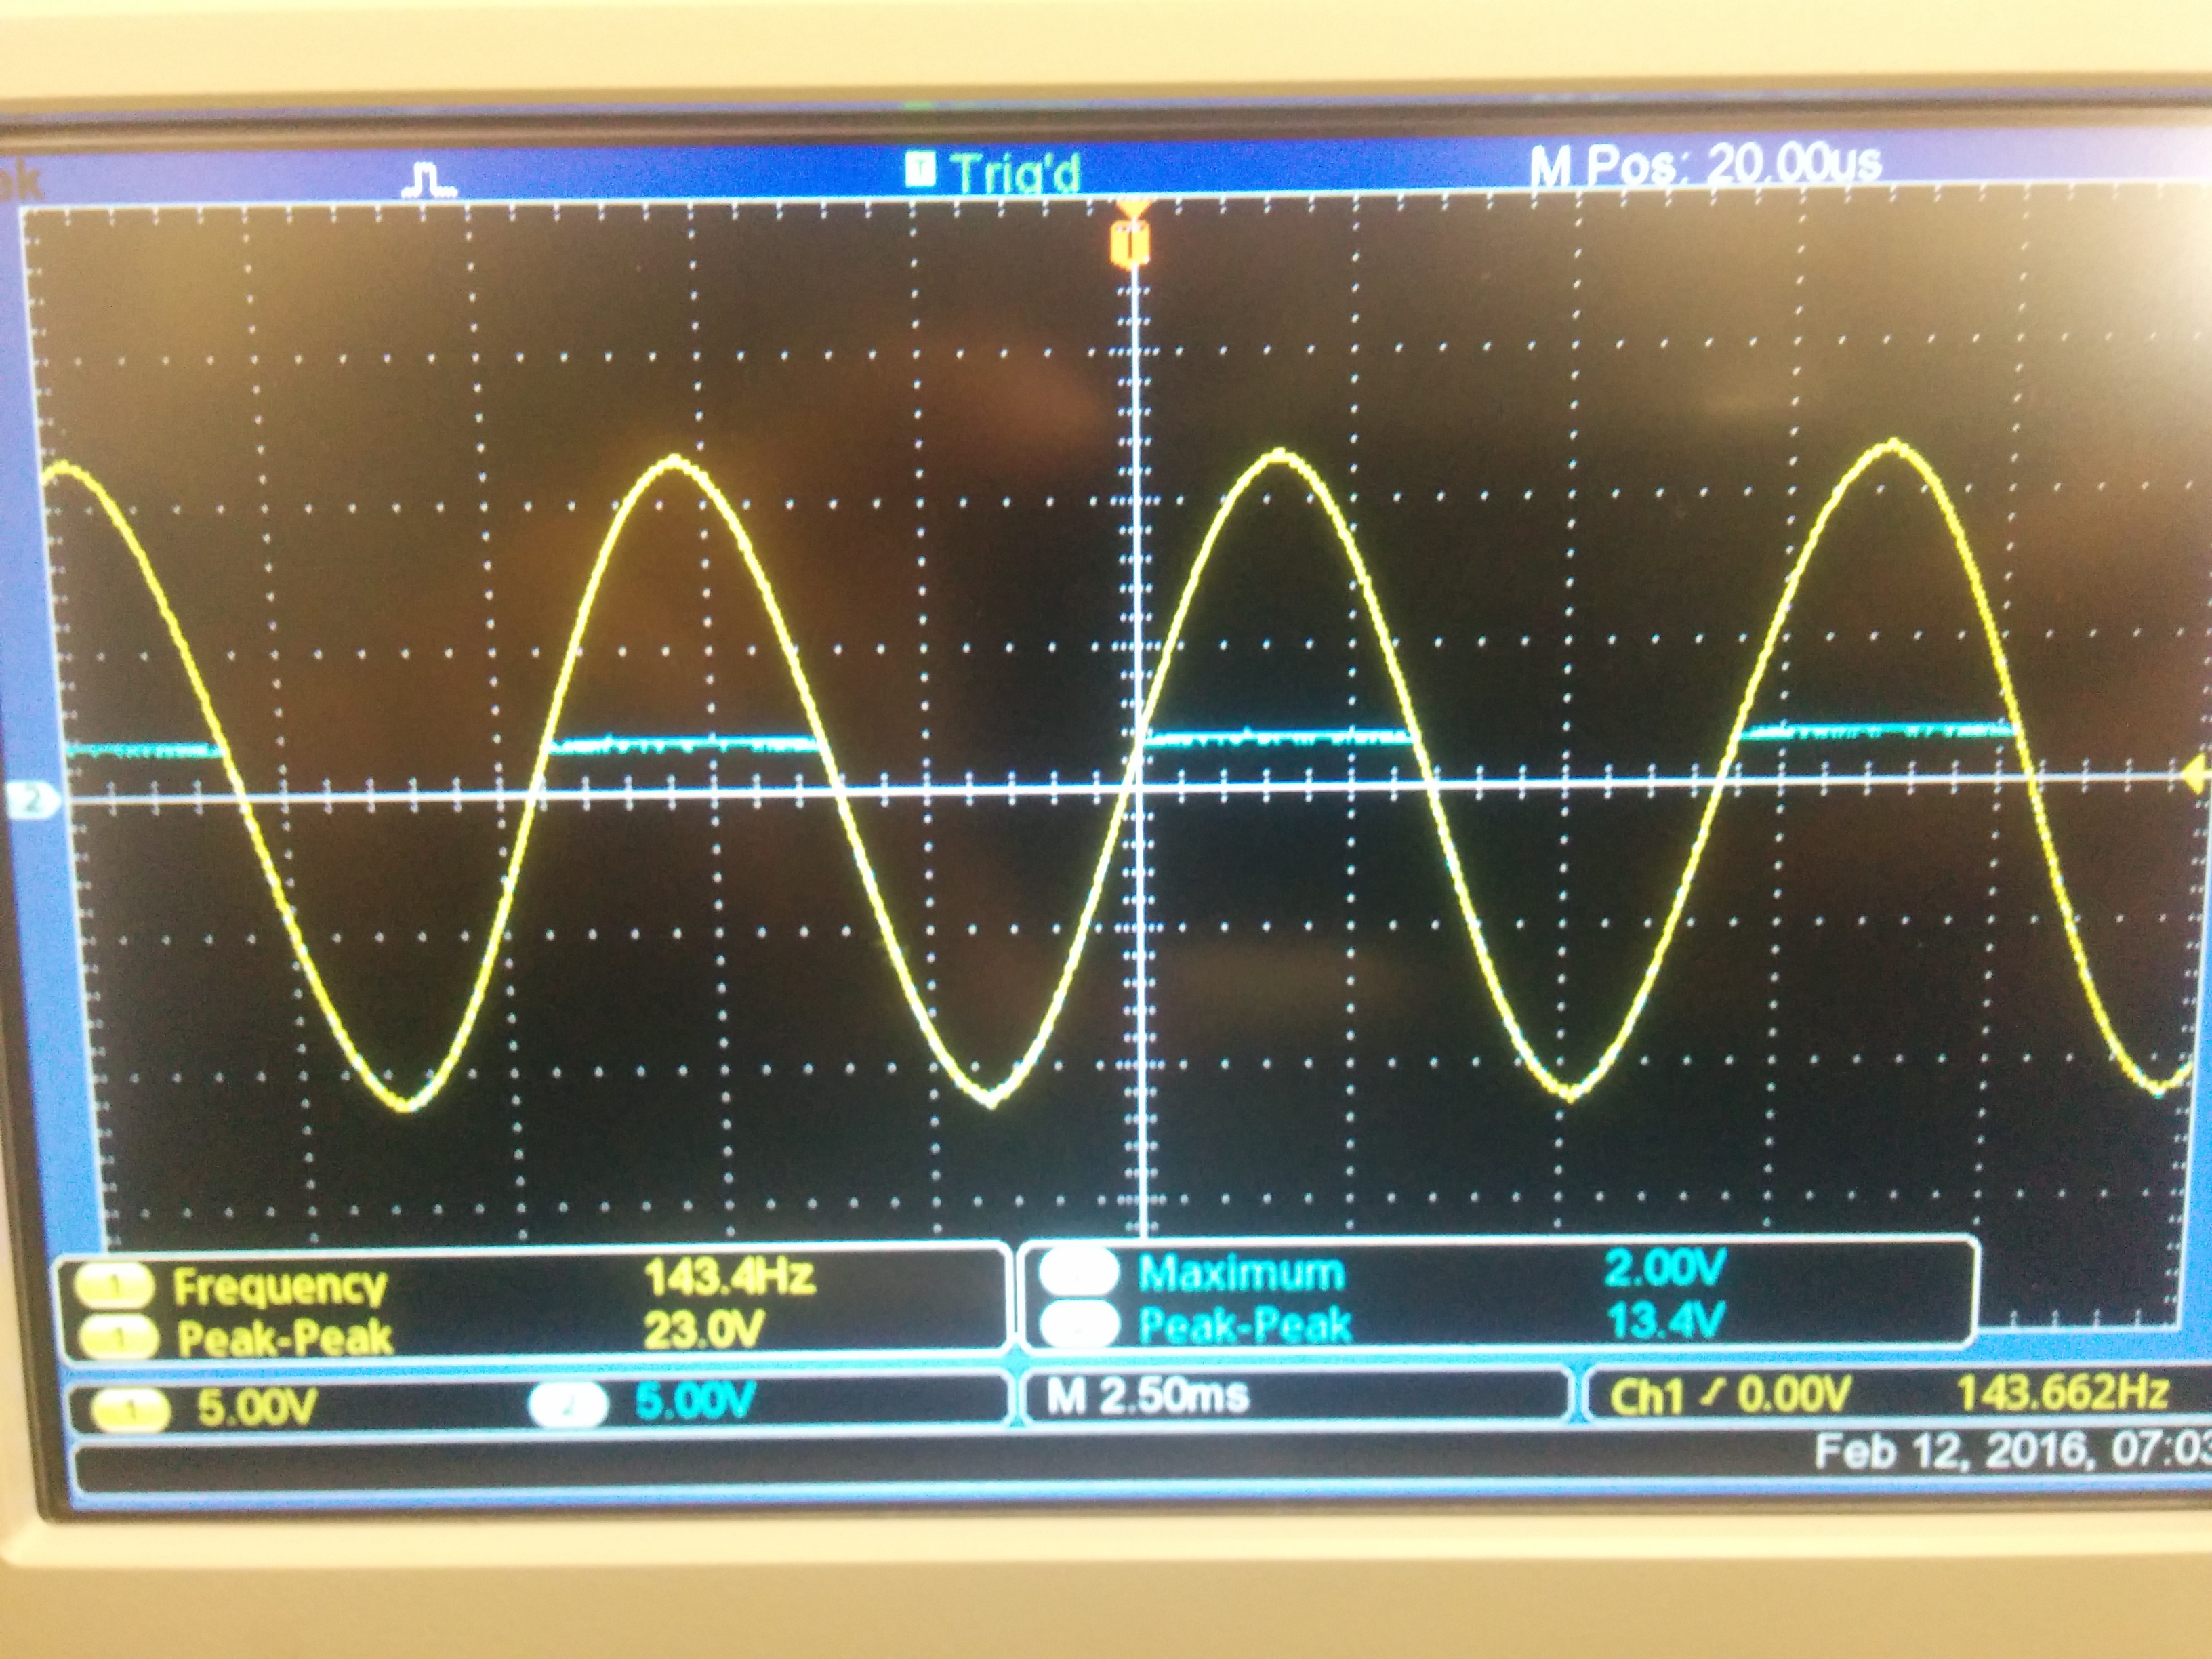
\includegraphics[scale =.1]{Forwardbias.jpg}
    \caption{Forward bias. Yellow for input voltage, blue for output voltage.}
    \label{fig:frwdb}
\end{figure}

\begin{figure}[H]
    \centering
    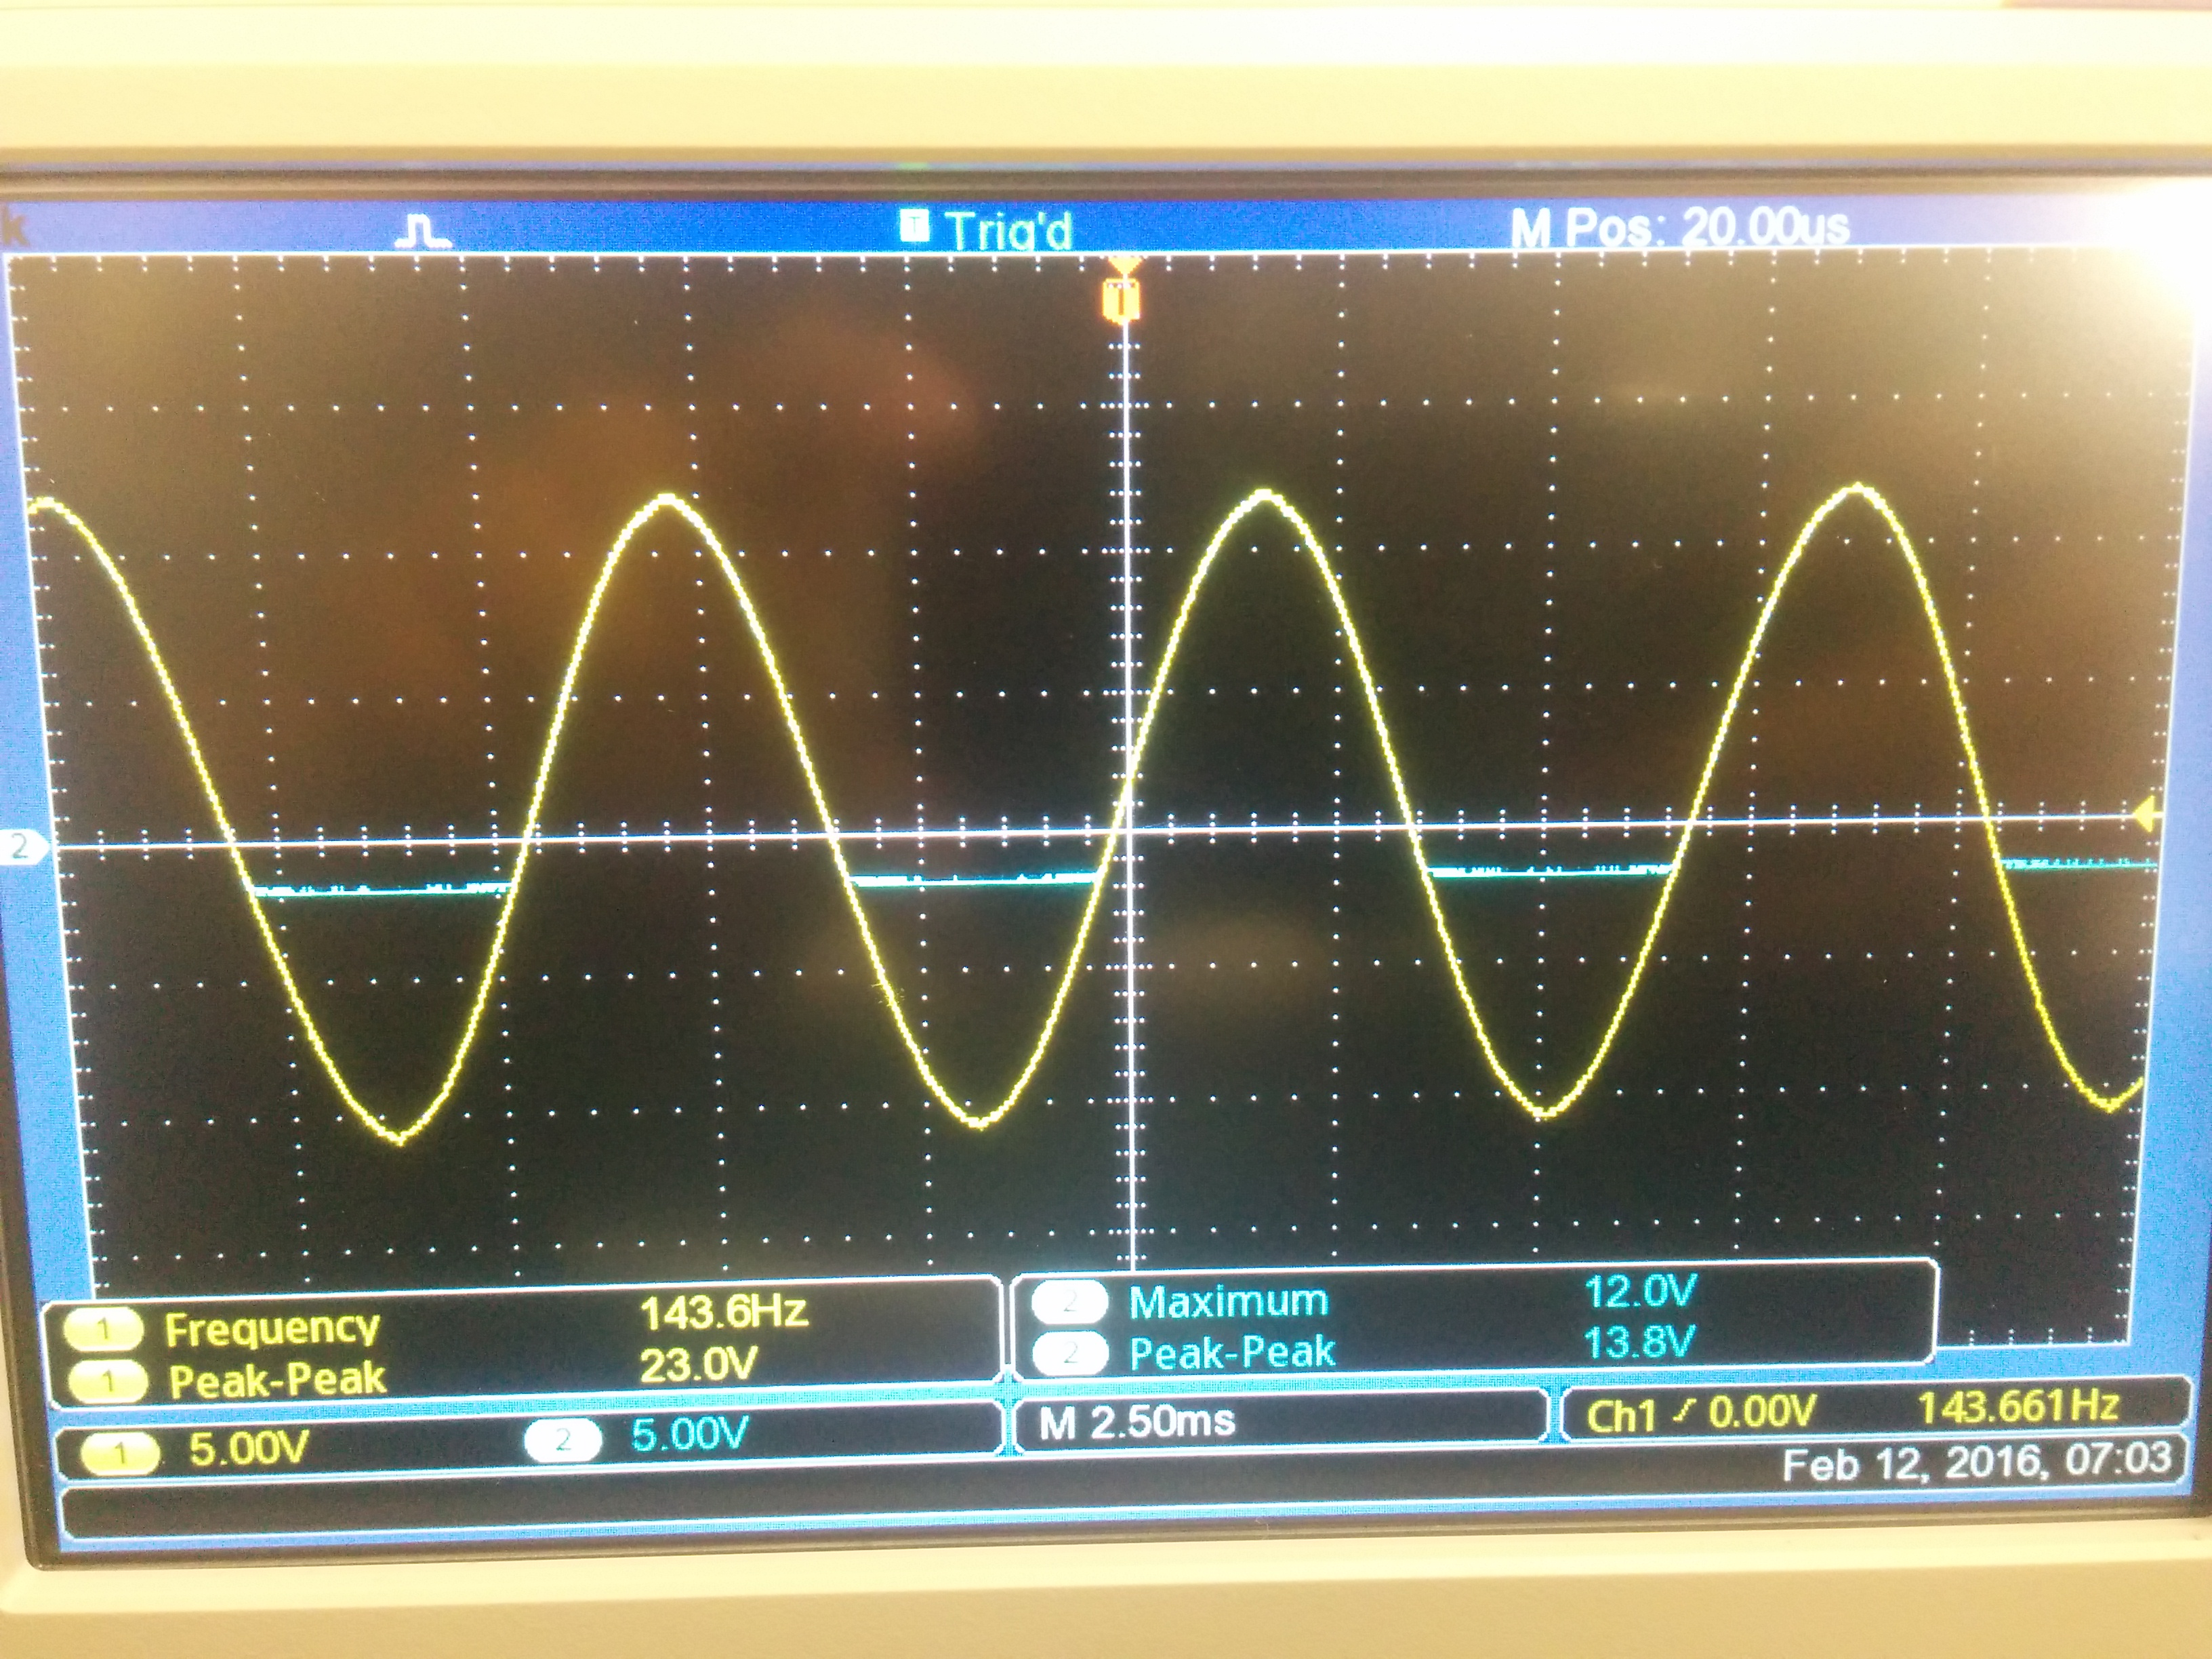
\includegraphics[scale =.1]{Reversebias.jpg}
    \caption{Reverse bias. Yellow for input voltage, blue for output voltage.}
    \label{fig:rvrsb}
\end{figure}

In order to observe the behavior in a LED, we simply set up a series 1K$\Omega$ resistor and the LED. We can see from fig. \ref{fig:frwdb} that the diode was in forward bias. We know this as the positive voltage is rectified while negative voltage is attenuated. In fig. \ref{fig:rvrsb}, we can see that the diode was in reverse bias. This follows the same reasoning as before: the negative voltage is rectified while positive voltage is attenuated. These trends can be verified thanks to fig. \ref{fig:graph}.0. In both directions there is a "breakdown" voltage that allows current to pass.  

\section{Summary and conclusions}

In this lab, we have seen that diodes rectify AC signals to DC both partially or completely. We also have seen that the diodes follow the expected behavior of fig. 2.0. Diodes are also responsive to AC signals in reverse and forward bias. In reverse bias, a diode acts as a high resistor preventing current from passing until the breakdown voltage. While in forward bias they allow current to pass more easily.  

Mathematically we can see that the diodes behavior is modeled by the shockley equation.
{\Large$$I = I_0(e^\frac{qV}{nkT}-1){\normalsize,}$$}

where I is the net current flow, $\mathrm{I_0}$ is the saturation current, q is the absolute value of the electron charge, V is the voltage across the diode, n is the ideal factor, k is Boltzmann's constant, and T is temperature.
Since our signal is an AC sine wave voltage, we can substitute the V with $V_0\sin{\omega t}$ for our signal. We can see that $e^{\sin{x}}$ produces a linear result.

%=====================================================
%============ Bibliography  ==============================
%=====================================================



%=====================================================
%============ End ====================================
%=====================================================

\end{document}

%=====================================================
%============ End ====================================
%=====================================================